\documentclass{article}
\usepackage[utf8]{inputenc}
\usepackage{geometry}
\usepackage{graphicx}
\usepackage{amsmath}
\usepackage{amsfonts}
\usepackage{amsthm}
\usepackage{amssymb}
\usepackage[most]{tcolorbox}
\usepackage{array}
\usepackage{latexsym}
\usepackage{alltt}
\usepackage{hyperref}
\usepackage{color, colortbl}
\usepackage{float}
\usepackage{pdfpages}
\usepackage{algpseudocode}
\usepackage{multicol}
\usepackage{multirow}
\usepackage{caption}
\usepackage{xparse}
\usepackage{setspace}
\usepackage{enumitem}
\usepackage{pdflscape}
% \usepackage{parskip}
\usepackage{blindtext}
\usepackage{forest}
\usepackage[newfloat]{minted}
\usepackage{booktabs}
\usepackage[graph,arrow,curve,color]{xy}


\geometry
{
  a4paper,
  left=12mm,
  right=12mm,
  top=12mm,
  bottom=15mm,
}

% mybox
\newtcolorbox{mybox}[3][]
{
  colframe = #2!25,
  colback  = #2!10,
  coltitle = #2!20!black,  
  title    = {#3},
  #1,
}

\definecolor{bg}{rgb}{0.95,0.95,0.95}
\setminted
{
	mathescape=true,
	xleftmargin=\parindent,
	bgcolor=bg,
  escapeinside=@@
}

\SetupFloatingEnvironment{listing}{name=Code}

\usetikzlibrary{patterns,positioning,fit,arrows,calc,shapes,decorations.pathreplacing,shadows,matrix}

% New environments that use mybox
\newcounter{example}[section]
\newenvironment{example}[1]{\begin{mybox}[breakable]{green}{\refstepcounter{example}\textbf{Example \thesection.\theexample #1}}}{\end{mybox}}

\newcounter{definition}[section]
\newenvironment{definition}[1]{\refstepcounter{definition}\begin{mybox}[breakable]{blue}{\textbf{Definition \thesection.\thedefinition #1}}}{\end{mybox}}

\newcounter{theorem}[section]
\newenvironment{theorem}[1]{\begin{mybox}{red}{\refstepcounter{theorem}\textbf{Theorem \thesection.\thetheorem #1}}}{\end{mybox}}

\newenvironment{formula}[1]{\begin{mybox}{cyan}{\textbf{#1}}}{\end{mybox}}

% Changing maketitle
\makeatletter         
\renewcommand\maketitle{
{\raggedright % Note the extra {
\begin{center}
{\Large \bfseries \@title}\\[2ex] 
{\large \@author \ - \@date}\\[2ex]
\end{center}}} % Note the extra }
\makeatother

% \onehalfspacing % adjust spacing
\setlength{\parskip}{0.5\baselineskip}

% macros
\newcommand{\prob}[1]{\textbf{\textit{P}}\left\{#1\right\}}
\newcommand{\expc}[1]{\mathbf{E}\left(#1\right)}
\newcommand{\expcs}[1]{\mathbf{E}^2\left(#1\right)}
\newcommand{\var}[1]{\text{Var}\left( #1 \right)}
\newcommand{\ra}{\rightarrow}
\newcommand{\Ra}{\Rightarrow}

\NewDocumentCommand{\dsum}{%
    e{^_}
}{%
  {% 
    \displaystyle\sum
    \IfValueT{#1}{^{#1}}
    \IfValueT{#2}{_{#2}}
  }
}%

% maketitle variables
\title{CENG 242 - Chapter 5: Procedural Abstraction (Abstraction)}
\author{Burak Metehan Tunçel}
\date{May 2022}

\begin{document}

\maketitle

\begin{multicols*}{2}
\setlength{\columnsep}{1.5cm}
\setlength{\columnseprule}{0.2pt}

\textbf{Abstraction:} Make a program or design reusable by enclosing it in a body, hiding the details, and defining a mechanism to access it. Main idea is separating the usage and implementation of program segments. It is vital in large scale programming. Abstraction is possible in any discipline involving design.

\paragraph*{Purpose}
\begin{itemize}
  \item Details are confusing
  \item Details may contain more error
  \item Repeating same details increase complexity and errors
  \item Abstraction philosophy: \textit{Declare once, use many times!}
  \item \textit{Code reusability} is the ultimate goal
  \item Parameterization improves power of abstraction
\end{itemize}


\section{Function Procedures and Proper Procedures}

A \textit{\textbf{procedure}} is an entity that embodies a computation. In particular, a \textit{function procedure} embodies an expression to be evaluated, and a \textit{proper procedure} embodies a command to be executed. The embodied computation is to be performed whenever the procedure is called.

A procedure is often defined by one programmer (the \textit{implementer}) and called by other programmers (the \textit{application programmers}). The application programmers are concerned only with the procedure's \textit{observable behavior}, in other words the outcome of calling the procedure. The implementer is concerned with how that outcome is to be achieved, in other words the choice of algorithm.

Note that the \textit{methods} of object-oriented languages are essentially procedures by another name. The only difference is that every method is associated with a class or with a particular object.

\subsection{Function Procedures}

A \textit{\textbf{function procedure}} (or simply \textit{function}) embodies an expression to be evaluated. When called, the function procedure will yield a value known as its \textit{result}. The application programmer observes only this result, not the steps by which it was computed.

\vspace*{\fill}
\columnbreak

\noindent A \texttt{C} or \texttt{C++} function definition has the form:
\begin{equation*}
  T\ I\ (FPD_1, \ldots, FPD_n)\ B
\end{equation*}
where
\begin{itemize}
  \item $I$ is the function’s identifier
  \item $FPD_i$ are \textit{formal parameter} declarations
  \item $T$ is the result type
  \item $B$ is a block command called the function's \textbf{body}.
\end{itemize}  
$B$ must contain at least one return of the form ``\textbf{return $E$};'', where $E$ is an expression of type $T$. The function procedure will be called by an expression of the form ``$I(AP_1, \ldots, AP_n)$;'', where the $AP_i$ are \textit{actual parameters}.

In general, a function call can be understood from two different points of view:
\begin{itemize}
  \item The \textit{application programmer}'s view of the function call is that it will map the arguments to a result of the appropriate type. Only this mapping is of concern to the application programmer.
  \item The \textit{implementer}'s view of the function call is that it will evaluate or execute the function's body, using the function's formal parameters to access the corresponding arguments, and thus compute the function's result. Only the algorithm encoded in the function's body is the implementer's concern.
\end{itemize}


\subsection{Proper Procedures}

A \textit{\textbf{proper procedure}} embodies a command to be executed, and when called will update variables. The application programmer observes only these updates, not the steps by which they were effected.

A \texttt{C} or \texttt{C++} proper procedure definition has the form:
\begin{equation*}
  \textbf{void}\ I\ (FPD_1, \ldots, FPD_n)\ B
\end{equation*}
where
\begin{itemize}
  \item $I$ is the function's identifier
  \item $FPD_i$ are the \textit{formal parameter} declarations
  \item $B$ is a block command called the procedure's \textit{\textbf{body}}.
\end{itemize}
The procedure will be called by a command of the form ``$I(AP_1, \ldots, AP_n)$;'', where the $AP_i$ are \textit{actual parameters}.

\vspace*{\fill}
\columnbreak

In general, a procedure call can be understood from two different points
of view:
\begin{itemize}
  \item The \textit{application programmer}'s view of the procedure call is its final outcome, which is that certain variables are updated. Only this outcome is of concern to the application programmer.
  \item The \textit{implementer}'s view of the procedure call is that it will execute the procedure's body, using the procedure's formal parameters to access the corresponding arguments. Only the algorithm encoded in the procedure's body is the implementer's concern.
\end{itemize}


\subsection{The Abstraction Principle}

We may summarize the preceding subsections as follows:
\begin{itemize}
  \item A \textit{function procedure} abstracts over an \textit{expression}. That is to say, a function procedure has a body that is an expression (at least in effect), and a function call is an expression that will yield a result by evaluating the function procedure's body.
  \item A \textit{proper procedure} abstracts over a command. That is to say, a proper procedure has a body that is a command, and a procedure call is a command that will update variables by executing the proper procedure's body.
\end{itemize}

Thus there is a clear analogy between function and proper procedures. We can extend this analogy to construct other types of procedures. The \textit{\textbf{Abstraction Principle}} states:
\begin{quote}
  \textit{It is possible to design procedures that abstract over any syntactic category, provided only that the constructs in that syntactic category specify some kind of computation.}
\end{quote}

\subsubsection{Selector Abstraction}

For instance, a variable access refers to a variable. We could imagine designing a new type of procedure that abstracts over variable accesses. Such a procedure, when called, would yield a variable. In fact, such procedures do exist, and are called \textit{\textbf{selector procedures}}:
\begin{itemize}
  \item A \textit{selector procedure} abstracts over a \textit{variable access}. That is to say, a selector procedure has a body that is a variable access (in effect), and a selector call is a variable access that will yield a variable by evaluating the selector procedure’s body.
\end{itemize}
Selector procedures are uncommon in programming languages, but they are
supported by \texttt{C++}. 

\vspace*{\fill}
\columnbreak

As an example, [..] is a operator that selects elements of an array. There can be user defined selectors on user defined structures.

\begin{listing}[H]

\begin{minted}{cpp}
struct List {
  int data;
  List *next;

  int &operator[](int el) {
    int i; List *p = this;
    for (i = 1 ; i < el ; i++) 
      p = p->next;  /* take the next element */
  
    return p->data;
  };
  ...
};

List h;
...
h[1] = h[2] + 1;
\end{minted}
\caption{}
\label{code:code1}
\end{listing}

In Python, \mintinline[bgcolor={}]{py}{__setitem__(k,v)} implements l-value, \mintinline[bgcolor={}]{py}{__getitem__(k,v)} r-value selector.

\begin{listing}[H]

\begin{minted}{py}
class BSTree:
  def __init__(self):
    self.node = None
  def __getitem__(self, key):
    if self.node == None:
        raise KeyError
    elif key < self.node[0]:
      return self.left[key]
    elif key > self.node[0]:
      return self.right[key]
    else:
      return self.node[1]
  def __setitem__(self, key, val):
    if self.node == None:
        self.node = (key,val)
        self.left = BSTree()    # empty tree
        self.right = BSTree()   # empty tree
    elif key < self.node[0]:
      self.left[key] = val
    elif key > self.node[0]:
      self.right[key] = val
    else:
      self.node = (key,val)

a = BSTree()
a["hello"] = 4
a["world"] = a["hello"] + 5
\end{minted}
\caption{}
\label{code:code2}
\end{listing}

\vspace*{\fill}
\columnbreak

\subsubsection{Generic Abstraction}

Another direction in which we might push the Abstraction Principle is to
consider whether we can abstract over \textit{declarations}. This is a much more radical idea, but it has been adopted in some modern languages such as \texttt{C++} and \texttt{JAVA}. We get a construct called a \textit{\textbf{generic unit}}:
\begin{itemize}
  \item A \textit{generic unit} abstracts over a \textit{declaration}. That is to say, a generic unit has a body that is a declaration, and a generic instantiation is a declaration that will produce bindings by elaborating the generic unit's body.
\end{itemize}

In other words, \textit{same declaration pattern applied to different data types}. A function or class declaration can be adapted to different types or values by using type or value parameters.
\begin{listing}[H]

\begin{minted}{cpp}
template <class T> class List {
	T content;
	List *next;
  public: List() { next = NULL };
	void add(T el) { ... };
	T get(int n) { ...};
};

template <class U>
  void swap(U &a, U &b)
    { U tmp; tmp=a; a=b; b=tmp; }
...
List<int> a; List<double> b; List<Person> c;
int t,x; double v,y; Person z,w;
swap(t,x); swap(v,y); swap(z,w);
\end{minted}
\caption{}
\label{code:code3}
\end{listing}

\subsubsection{Iterator Abstraction}

Iteration over a user defined data structure. Python generator example:
\begin{listing}[H]

\begin{minted}{py}
class BSTree(object):
  def __init__(self):
    self.val = ()
  def inorder(self):
    if self.val == ():
      return
    else:
      for i in self.left.inorder():
        yield i
      yield self.val
      for i in self.right.inorder():
        yield i

v = BSTree()
...
for v in v.inorder():
  print v
\end{minted}
\caption{}
\label{code:code4}
\end{listing}

\paragraph{C++ Iterators}
\texttt{C++} Standard Template Library containers support \textit{iterators} \mintinline{cpp}{begin()} and \mintinline{cpp}{end()} methods return iterators to start and end of the data structure. Iterators can be dereferenced as \mintinline{cpp}{*iter} or \mintinline{cpp}{iter->member}.`\mintinline{cpp}{++}' operation on an iterator skips to the next value.
\begin{listing}[H]
\begin{minted}{cpp}
for (@$\textit{ittype}$@ it = a.begin(); it != a.end(); ++it) {
  // use *it or it->member it->method() in body
}
\end{minted}
\end{listing}
\texttt{C++11} added:
\begin{listing}[H]
\begin{minted}{cpp}
for (@$\textit{valtype}$@ & i : a ) {
  // use directly i as l-value or r-value. 
}
\end{minted}
\end{listing}
This syntax is equivalent to:
\begin{listing}[H]
\begin{minted}{cpp}
for (@$\textit{ittype}$@ it = a.begin() ; it != a.end(); it++) {
  @$\textit{valtype}$@ & i = *it;
  // use directly i as l-value or r-value 
}
\end{minted}
\end{listing}
Following is the general examples:
\begin{listing}[H]

\begin{minted}{cpp}
template<class T>
class List {
  struct Node { T val; Node *next;} *list;
public:
  List() { list = nullptr;}
  void insert(const T& v) { 
    Node *newnode = new Node;
    newnode->next = list; newnode->val = v; 
    list = newnode;
  }
  class Iterator {
    Node *pos;
  public: 
    Iterator(Node *p) { pos = p; }
    T & operator*() { return pos->val; }
    void operator++() { pos = pos->next; }
    bool operator!=(const Iterator &it) { 
      return pos != it.pos;
    }
  };
  
  Iterator begin() 
    { Iterator it = Iterator(list); return it; }
  Iterator end()
    { Iterator it = Iterator(nullptr); return it; }
};
List<int> a;
// C++11 syntax below
for (int & i : a )
  i *= 2; cout << i << '\n';
\end{minted}
\caption{}
\label{code:code5}
\end{listing}

\subsection{Abstraction Principle}

If any programming language entity involves computation, it is possible to define an abstraction over it

\begin{center}
  \begin{tabular}{l!{$\rightarrow$}l}\rowcolor{blue!10!white}
  \bf Entity & \bf Abstraction \\
  \rowcolor{blue!5!white} Expression	& Function \\
  \rowcolor{blue!5!white} Command  & Procedure \\
  \rowcolor{blue!5!white} Selector & Selector function \\
  \rowcolor{blue!5!white} Declaration  & Generic \\
  \rowcolor{blue!5!white} Command Block & Iterator \\
  \end{tabular}
\end{center}


\section{Parameters and Arguments}

An \textit{\textbf{argument}} is a value or other entity that is passed to a procedure. An \textit{\textbf{actual parameter}} is an expression (or other construct) that yields an argument. A \textit{\textbf{formal parameter}} is an identifier through which a procedure can access an argument.

In all programming languages, \textit{first-class values can be passed as arguments}. In most languages, \textit{either variables or pointers to variables can be passed as arguments}. In some languages, \textit{either procedures or pointers to procedures can be passed as arguments}.

When a procedure is called, each formal parameter will become associated, in some sense, with the corresponding argument. The nature of this association is called a \textit{\textbf{parameter mechanism}}. Parameter mechanisms can be understood in terms of two basic concepts:
\begin{itemize}
  \item A \textit{copy parameter} mechanism binds the formal parameter to a local variable that contains a copy of the argument.
  \item A \textit{reference parameter} mechanism binds the formal parameter directly to the argument itself.
\end{itemize}

\subsection{Copy Parameter Mechanisms}

A \textit{\textbf{copy parameter mechanism}} allows for a value to be copied into and/or out of a procedure. The formal parameter $FP$ denotes a local variable of the procedure. A value is copied into $FP$ on calling the procedure, \textit{and/or} is copied out of $FP$ (to an argument variable) on return. The local variable is created on calling the procedure, and destroyed on return.

\noindent There are three possible copy parameter mechanisms:
\begin{itemize}
  \item A \textit{\textbf{copy-in parameter}} (also known as a \textit{value parameter}) works as follows. When the procedure is called, a local variable is created and initialized with the argument value. Inside the procedure, that local variable may be inspected and even updated. (However, any updating of the local variable
  has no effect outside the procedure.)
  \item A \textit{\textbf{copy-out parameter}} (also known as a \textit{result parameter}) is a mirror-image of a copy-in parameter. In this case the argument must be a variable. When the procedure is called, a local variable is created but not initialized. When the procedure returns, that local variable's final value is assigned to the argument variable.
  \item A \textit{\textbf{copy-in-copy-out parameter}} (also known as a \textit{value-result parameter}) combines copy-in and copy-out parameters. In this case also, the argument must be a variable. When the procedure is called, a local variable is created and initialized with the argument variable's current value. When the procedure returns, that local variable's final value is assigned back to the argument variable.
\end{itemize}
\texttt{C}, \texttt{C++}, and \texttt{JAVA} support \textit{only} copy-in parameters.

\subsection{Reference Parameter Mechanisms}

A \textit{\textbf{reference parameter mechanism}} allows for the formal parameter $FP$ to be bound directly to the argument itself.

\noindent Reference parameter mechanisms appear under several guises in programming languages:
\begin{itemize}
  \item In the case of a \textit{\textbf{constant parameter}}, the argument must be a value. $FP$ is bound to the argument value during the procedure's activation. Thus any inspection of $FP$ is actually an indirect inspection of the argument value.
  \item In the case of a \textit{\textbf{variable parameter}}, the argument must be a variable. $FP$ is bound to the argument variable during the procedure's activation. Thus any inspection (or updating) of $FP$ is actually an indirect inspection (or updating) of the argument variable.
  \item In the case of a \textit{\textbf{procedural parameter}}, the argument must be a procedure. $FP$ is bound to the argument procedure during the called procedure's activation. Thus any call to $FP$ is actually an indirect call to the argument procedure.
\end{itemize}
\texttt{C++} does support variable parameters directly. If the type of a formal parameter is $T\&$ (reference to $T$), the corresponding argument must be a variable of type $T$.

The choice between reference and copy parameter mechanisms is an important decision for the language designer. Reference parameters have simpler semantics, and are suitable for all types of value (including procedures, which in most programming languages cannot be copied). Reference parameters rely on indirect access to argument data, so \textit{copy parameters are more efficient for primitive types, while reference parameters are usually more efficient for composite types}. (In a distributed system, however, the procedure might be running on a processor remote from the argument data, in which case it may be more efficient to copy the data and then access it locally.)

A disadvantage of variable parameters is that aliasing becomes a hazard. \textit{\textbf{Aliasing}} occurs when two or more identifiers are simultaneously bound to the same variable (or one identifier is bound to a composite variable and a second identifier to one of its components). Aliasing tends to make programs harder to understand and harder to reason about.

\end{multicols*}

\begin{multicols}{2}
\setlength{\columnsep}{1.5cm}
\setlength{\columnseprule}{0.2pt}
\subsection{The Correspondence Principle}

You might have noticed a correspondence between certain parameter mechanisms and certain forms of declaration. For example:
\begin{itemize}
  \item A \textit{constant parameter} corresponds to a \textit{constant definition}. In each case, an identifier is bound to a first-class value.
  \item A \textit{variable parameter} corresponds to a \textit{variable renaming definition}. In each case, an identifier is bound to an existing variable.
  \item A \textit{copy-in parameter} corresponds to an \textit{(initialized) variable declaration}. In each case, a new variable is created and initialized, and an identifier is bound to that variable.
\end{itemize}

\noindent The \textit{\textbf{Correspondence Principle}} states:
\begin{quote}
  \textit{For each form of declaration there exists a corresponding parameter mechanism.}
\end{quote}
Note that the converse is not always true.

\noindent \texttt{C}:
\begin{table}[H]
  \centering
  \begin{tabular}{>{\tt}l!{$\leftrightarrow$}>{\tt}l}
    \rowcolor{blue!5!white}
      \mintinline[bgcolor={}]{c}{int a = p;} & \mintinline[bgcolor={}]{c}{void f(int a) {...}} \\
    \rowcolor{blue!10!white}
      \mintinline[bgcolor={}]{c}{const int a = p;} & \mintinline[bgcolor={}]{c}{void f(const int a) {...}}
  \end{tabular}
\end{table}


\noindent \texttt{Pascal}:
\begin{table}[H]
  \centering
  \begin{tabular}{>{\tt}l!{$\leftrightarrow$}>{\tt}l}
    \rowcolor{blue!5!white}
      var a: integer; & procedure f(a:integer) \\
    \rowcolor{blue!5!white}
      & begin\\
    \rowcolor{blue!10!white} 
      const a: 5; & ??? \\
    \rowcolor{blue!5!white}
      ???	    & procedure f(var a:integer)\\
    \rowcolor{blue!5!white}
      & begin
  \end{tabular}
\end{table}

\noindent \texttt{C++}:
\begin{table}[H]
  \centering
  \begin{tabular}{>{\tt}l!{$\leftrightarrow$}>{\tt}l}
    \rowcolor{blue!5!white}
      \mintinline[bgcolor={}]{cpp}{int a = p;} & \mintinline[bgcolor={}]{cpp}{void f(int a) {...}} \\
    \rowcolor{blue!10!white}
      \mintinline[bgcolor={}]{cpp}{const int a = p;} & \mintinline[bgcolor={}]{cpp}{void f(const int a) {...}}\\
    \rowcolor{blue!5!white}
      \mintinline[bgcolor={}]{cpp}{&a = p} & \mintinline[bgcolor={}]{cpp}{void f(int &a) {...}}
  \end{tabular}
\end{table}

\vspace*{\fill}
\columnbreak


\section{Parameters (\textit{from slides})}

\textbf{Declaration part:}

\texttt{abstraction\_name $(FP_1, FP_2, \ldots, FP_n)$}

\noindent \textbf{Use part:}

\texttt{abstraction\_name $(AP_1, AP_2, \ldots, AP_n)$}

\noindent \textit{\textbf{Formal parameters:}} Identifiers or constructors of identifiers (patterns in functional languages).

\noindent \textit{\textbf{Actual parameters:}} Expression or identifier based on the type of the abstraction and parameter.

\subsection{Parameter passing mechanisms}

Programming language may support one or more mechanisms. 3 basic methods:
\begin{enumerate}
 \item Copy mechanisms (assignment based)
 \item Binding mechanisms 
 \item Pass by name (substitution based)
\end{enumerate}

\subsubsection{Copy Mechanisms}

Function and procedure abstractions, assignment between actual and formal parameter:
\begin{enumerate}
 \item \textbf{Copy In:} \\
	On function call: $FP_i \leftarrow AP_i$
 \item \textbf{Copy Out:} \\
	On function return: $AP_i \leftarrow FP_i$
 \item \textbf{Copy In-Out:} \\
	On function call: $FP_i \leftarrow AP_i$, and\\
	On function return: $AP_i \leftarrow FP_i$
\end{enumerate}
\texttt{C} only allows copy-in mechanism. This mechanism is also called as \textbf{Pass by value}.

\end{multicols}

\begin{minipage}{.29\linewidth}

\begin{listing}[H]

\begin{minted}{c}
int x=1, y=2;
void f(int a, int b) {
  x += a+b;
  a++;
  b=a/2;
}

int main() {
  f(x,y);
  printf("x:%d, y:%d\n",x,y);
  return 0;
}
\end{minted}
\caption{}
\label{code:code6}
\end{listing}

\end{minipage}%
\begin{minipage}{.05\linewidth}
  \vspace*{\fill}
  \hspace*{\fill}
\end{minipage}%
\begin{minipage}{.29\linewidth}

  \underline{\textbf{Copy In:}}

  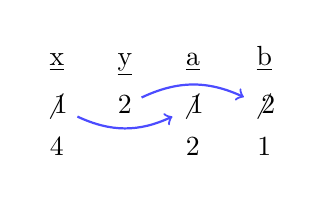
\begin{tikzpicture}
  \matrix [matrix of nodes,nodes in empty cells,ampersand replacement=\&,column sep=4mm] (m) {
      \underline{x} \&\underline{y} \&\underline{a} \&\underline{b} \\
          {$\not 1$} \& {$2$} \& {$\not 1$} \& {$\not 2$} \\ 
  $4$ \&  \&  $2$ \& $1$ \\
  };
  \draw [bend right=25,->,thick,blue!70!white] (m-2-1) to (m-2-3); 
  \draw [bend left=25,->,thick,blue!70!white] (m-2-2) to (m-2-4); 
  \end{tikzpicture}

  \texttt{x:4, y:2}

  \underline{\textbf{Copy Out:}}

  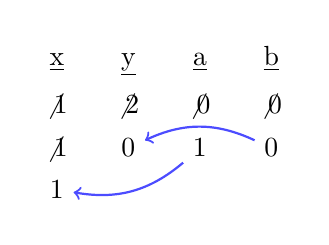
\begin{tikzpicture}
  \matrix [matrix of nodes,nodes in empty cells,ampersand replacement=\&,column sep=4mm] (m) {
  \underline{x} \&\underline{y} \&\underline{a} \&\underline{b} \\
  $\not 1$ \& $\not 2$ \& $\not 0$ \& $\not 0$ \\
  $\not 1$      \&  {$0$}   \& {$1$}  \& {$0$} \\
  {$1$} \& \& \& \\ 
  };
  \draw [bend left=25,->,thick,blue!70!white] (m-3-3) to (m-4-1); 
  \draw [bend right=25,->,thick,blue!70!white] (m-3-4) to (m-3-2); 
  \end{tikzpicture}

  \texttt{x:1, y:0}

\end{minipage}%
\begin{minipage}{.05\linewidth}
  \vspace*{\fill}
  \hspace*{\fill}
\end{minipage}%
\begin{minipage}{.29\linewidth}

  \underline{\textbf{Copy In-Out:}}

  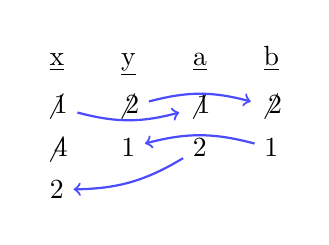
\begin{tikzpicture}
  \matrix [matrix of nodes,nodes in empty cells,ampersand replacement=\&,column sep=4mm] (m) {
  \underline{x} \&\underline{y} \&\underline{a} \&\underline{b} \\
  {$\not 1$} \& {$\not 2$} \& {$\not 1$} \& {$\not 2$} \\ 
  $\not 4$ \&  {$1$}\&  {$2$} \& {$1$} \\
  {$2$} \\
  };
  \draw [bend right=15,->,thick,blue!70!white] (m-2-1) to (m-2-3); 
  \draw [bend left=15,->,thick,blue!70!white] (m-2-2) to (m-2-4); 
  \draw [bend left=15,->,thick,blue!70!white] (m-3-3) to (m-4-1); 
  \draw [bend right=15,->,thick,blue!70!white] (m-3-4) to (m-3-2); 
  \end{tikzpicture}

  \texttt{x:2, y:1}

\end{minipage}

\subsubsection{Binding Mechanisms}

Based on binding of the formal parameter variable/identifier to actual parameter value/identifier. Only one entity (value, variable, type) exists with more than one names.
\begin{enumerate}
  \item \textbf{Constant binding:} Formal parameter is constant during the function. The value is bound to actual parameter expression value. \\
  Functional languages including Haskell uses this mechanism.
  \item \textbf{Variable binding:} Formal parameter variable is bound to the actual parameter variable. Same memory area is shared by two variable references.\\  
  Also known as \textbf{pass by reference}.
\end{enumerate}
The other type and entities (function, type, etc) are passed with similar mechanisms. 

\begin{minipage}{.4\linewidth}

\begin{listing}[H]
\begin{minted}{c}
int x = 1, y = 2;
void f(int a, int b) {
  x += a + b;
  a++;
  b = a / 2;
}

int main() {
  f(x, y);
  printf("x:%d , y:%d\n",x,y);
  return 0;
}
\end{minted}
\caption{}
\label{code:code7}
\end{listing}

\end{minipage}%
\begin{minipage}{.1\linewidth}
  \vspace*{\fill}
  \hspace*{\fill}
\end{minipage}%
\begin{minipage}{.4\linewidth}
  \underline{\textbf{Variable binding:}}\\
  \begin{tabular}{cp{.5em}c}
    f():a & & f():b \\
    x & & y \\ \cline{1-1} \cline{3-3}
    $\not 1$ 		& &  	$\not 2$	\\
    $\not 4$ 		& &  	$2$	\\
    $5$ 			& &  		\\
  \end{tabular}\\
  \texttt{x: 5, y:2}
\end{minipage}

\subsubsection{Pass by Name}

Actual parameter syntax replaces each occurence of the formal parameter in the function body, then the function body evaluated. \texttt{C} macros works with a similar mechanism (by pre-processor).

\noindent Mostly useful in theoretical analysis of PL's. Also known as \textbf{Normal order evaluation}.

Example (Haskell-like)
\begin{listing}[ht]

\begin{minted}{haskell}
f x y = if (x < 12) then x*x + y*y + x 
        else x + x*x
\end{minted}

\caption{}
\label{code:code8}
\end{listing}

\noindent \textbf{Evaluation:}
\begin{align*}
  &\texttt{f } (3*12 + 7)\ (24 + 16*3) \\
  &\mapsto \texttt{if } ((3*12 + 7) < 12) \texttt{ then } (3*12 + 7) * (3*12 + 7) + (24 + 16*3) * (24 + 16*3) + (3*12 + 7)\\
  &\quad\ \ \ \ \texttt{else } (3*12 + 7) + (3*12 + 7) * (3*12 + 7)\\
  &\stackrel{*}{\mapsto} \texttt{if } (43 < 12) \texttt{ then } ...\\
  &\mapsto \texttt{if } (false) \texttt{ then } ...\\
  &\mapsto (3*12 + 7) + (3*12 + 7) * (3*12 + 7)\\
  &\stackrel{*}{\mapsto} (3*12 + 7) + 43 * (3*12 + 7)\\
  &\mapsto ... \mapsto 1892\quad \texttt{\textcolor{blue}{12 steps}}
\end{align*}

\noindent \textbf{Normal order evaluation} is mathematically natural order of evaluation.

\newpage

Most of the PL's apply \textit{\textbf{eager evaluation}}: Actual parameters are evaluated first, then passed.
\begin{align*}
  &\texttt{f } (3*12+7)\ (24+16*3) \\
  &\mapsto \texttt{f } (36+7)\ (24+16*3) \\
  &\stackrel{*}{\mapsto} \texttt{f } 43\ 72 \\
  &\mapsto \texttt{if } (43 < 12) \texttt{ then } 43*43 + 72*72 + 43 \\
  &\quad\ \ \texttt{else } 43+43*43\\
  &\mapsto \texttt{if } (false)\ \texttt{then } ...\\
  &\mapsto 43 + 43*43 \stackrel{*}{\mapsto} 1892 \quad \texttt{\textcolor{blue}{8 steps}}
\end{align*}

\noindent \textbf{Church–Rosser Property:} 
\begin{quote}
  If an expression can be evaluated at all, it can be evaluated by consistently using normal-order evaluation. If an expression can be evaluated in several different orders (mixing eager and normal-order evaluation), then all of these evaluation orders yield the same result.
\end{quote}

\noindent In $\lambda$-calculus, all orders reduce the same normal form.
\begin{center}
  
\xygraph{[]!{<20mm,0mm>:<0mm,12mm>::}
{\lambda x.(\lambda y.y+(\lambda x.x+1~y)~~(x+2))~~5}
 ( :@{|->}[dll] {\lambda y.y+(\lambda x.x+1~~y)~~(5+2)}
    ( :@{|->}[dl] {5+2+(\lambda x.x+1~~(5+2))}
        ( :@{|->}[ddddrrr] {5+2+5+2+1}="bot" ) ,
      :@{|->}@(dr,ur)[dddl] {\lambda y.y+y+1~~(5+2)} :@{|->}"bot"
    ),
   :@{|->}[dd]  {\lambda x.x+2+(\lambda x.x+1~~(x+2))~5}
    (
    :@{|->}[dl]  {5+2+(\lambda x.x+1~~(5+2))} :@{|->}"bot",
    :@{|->}[dr]  {\lambda x.x+2+x+2+1~~5} :@{|->}"bot"
    ),
   :@{|->}[drr] {\lambda x.(\lambda y.y+y+1~~(x+2))~~5} (
       :@{|->}[ddr] {\lambda y.y+y+1~~(5+2)} :@{|->}@(dr,r)"bot",
       :@{|->}[ddd] {\lambda x.x+2+x+2+1~~5} :@{|->}"bot")
 )
}

\end{center}

\noindent Haskell implements \textbf{Lazy Evaluation} order.
\begin{itemize}
  \item Eager evaluation is faster than normal order evaluation but violates Church-Rosser Property.
  \item Lazy evaluation is as fast as eager evaluation but computes same results with normal order evaluation (unless there is a side effect).
\end{itemize}
Lazy evaluation expands the expression as normal order evaluation however once it evaluates the formal parameter value other evaluations use previously found value:
\begin{align*}
  &\texttt{f } (3*12 + 7)\ (24 + 16*3)\\
  &\mapsto \texttt{if } (x:(3*12 + 7) < 12) \texttt{ then } x:(3*12 + 7) * x:(3*12 + 7) + y:(24 + 16*3) * y:(24 + 16*3) + x:(3*12+7)\\
  &\quad\ \ \texttt{else } x:(3*12 + 7) + x:(3*12 + 7) * x:(3*12 + 7)\\
  &\stackrel{*}{\mapsto} \texttt{if } (x:43 < 12) \texttt{ then } x:43 * x:43 + y:(24 + 16*3) * y:(24 + 16*3) + x:43\\
  &\quad\ \ \ \texttt{else } x:43 + x:43 * x:43\\
  &\mapsto \texttt{if } (false) \texttt{ then } ...\\
  &\mapsto x:43 + x:43 * x:43\\
  &\mapsto x:43 + 1849 \mapsto 1892 \quad \texttt{\textcolor{blue}{7 steps}}
\end{align*}
In lazy evaluation, parameters are passed by name but compiler keeps evaluation state of them. Parameter value is store once it is evaluated. Further evaluations use that.v

Python implementation. First delay evaluation of expressions. Convert to functions:

\lstinline!exp! $\rightarrow$ \lstinline[language=Python]!lambda : exp! \\
$\eta$ expansion. Function version is also called \textbf{thunk}.

Inside function, call these functions to evaluate the expression
\begin{listing}[ht]

\begin{minted}{py}
def E(thunk):
  if not hasattr(thunk,"stored"):
    thunk.stored = thunk()      # evaluate and store
  return thunk.stored           # use stored value
def f(x,y):
  if E(x) < 10:                # call E() on all evaluations
    return E(x)*E(x)+E(y)
  else:
    return E(x)*E(x)+E(x)
f(lambda : 3*32+4, lambda: 4/0)     # call by converting to function
\end{minted}

\caption{}
\label{code:code9}
\end{listing}v

Delayed evaluation in normal order or lazy evaluation enables working on infinite values.


% \section{Evaluation Order}

The slides also contain ``Evaluation Order''. This topic can be studied from slides or read from the textbook page 368.

\end{document}